\documentclass[11pt, aspectratio=169]{beamer}

\usepackage[utf8]{inputenc}
\usepackage{graphicx}
\usepackage{xcolor}
\usepackage{listings}
\usepackage{ragged2e} % Import the package
\usepackage{tikz}
\usepackage{caption}
\usepackage{biblatex}
\usepackage{url}
\usepackage{gospel}
\usepackage{bold-extra}
\usepackage{latexsym}
\usepackage{subcaption}
\usepackage{pgfplots}
\pgfplotsset{compat=1.18} % Or adjust based on your TeX version
\addbibresource{refs.bib}  % your bibliography file

\counterwithin{figure}{section}
\usetikzlibrary{arrows}
\usetikzlibrary{calc, positioning} % For coordinate calculations and relative positioning
\usetikzlibrary{
  chains,
  shapes,
  arrows.meta % supersedes the arrows library
}

\usetheme{Copenhagen}
\usecolortheme{default}

\setbeamertemplate{navigation symbols}{}
\setbeamertemplate{caption}[numbered]

\definecolor{codebg}{rgb}{0.95,0.95,0.95}

%%%%%%%%%%%%%%%%%%%%%%%%%%%%%%%%%%%%%%%%%%%%%%%%%%%%%%
%%%%%%% BAR UP TOP WITH THE SECTIONS %%%%%%%%%%%%%%%%%
%%%%%%%%%%%%%%%%%%%%%%%%%%%%%%%%%%%%%%%%%%%%%%%%%%%%%%

\useoutertheme[subsection=false]{miniframes}
\setbeamercolor{below lower separation line head}{bg=white}
\addtobeamertemplate{headline}{}{%
  \begin{beamercolorbox}[colsep=0pt]{below lower separation line head}
  \end{beamercolorbox}
}

%%%%%%%%%%%%%%%%%%%%%%%%%%%%%%%%%%%%%%%%%%%%%%%%%%%%%
%%%%%%%%% TO REMOVE ANY BARS UP TOP JUST UNCOMMENT%%%
%%%%%%%%%%%%%%%%%%%%%%%%%%%%%%%%%%%%%%%%%%%%%%%%%%%%%

% \setbeamertemplate{headline}{}

%%%%%%%%%%%%%%%%%%%%%%%%%%%%%%%%%%%%%%%%%%%%%%%%%%%%%

\setbeamercolor*{mini frame}{fg=white,bg=blue}
\setbeamercolor{section in head/foot}{fg=white}

\setbeamertemplate{footline}[frame number]

\definecolor{mykeyword}{rgb}{0.86, 0.078, 0.24}
\definecolor{mykeyword2}{rgb}{1, 0.65, 0}
\definecolor{mykeyword3}{rgb}{0, 0, 0.8}
\definecolor{mycomment}{rgb}{0.5, 0.5, 0.5} 
\definecolor{mystring}{rgb}{0.6, 0.0, 0.3}

\newcounter{figureNum}
\renewcommand{\thefigure}{\arabic{figureNum}}

\DeclareCaptionFormat{listing}{\hfill#3}
\captionsetup[lstlisting]{format=listing,singlelinecheck=false,
margin=0pt, font={sf,it},labelsep=space,labelfont=bf,belowskip=-1pt}

\title{\textbf{A Compositional Deadlock Detector for Android Java}}
\author{Darius Muresan \\[0.3em] Henrique Luz \\[0.1em] Rui Xavier}
\institute{Aarhus University \\ Department of Computer Science}
\date{November 11, 2025}

\setbeamertemplate{title page}{
  \vbox{}
  \vfill
  \begingroup
    \centering
    \usebeamertemplate{title}
    \vskip0.5em
    \usebeamertemplate{author}
    \usebeamertemplate{institute}
    \usebeamertemplate{date}
    \begin{center}
        \includegraphics[width=3.6cm]{LOGO DI.png}
    \end{center}
  \endgroup
  \vfill
}

\begin{document}

\newcommand{\nbnote}[3]{
  % \fbox{\bfseries\sffamily\scriptsize#1}
  \fcolorbox{gray}{yellow}{\bfseries\sffamily\scriptsize#1}
  {\color{#2} \sffamily\small$\blacktriangleright$\textit{#3}$\blacktriangleleft$}
  % {\color{#2} \sffamily\small$\textit{#3}$}
  % \marginpar{\fbox{\bfseries\sffamily#1}}
}

\newcommand{\mario}[1]{\nbnote{Mário}{red}{#1}}
%\renewcommand{\mario}[1]{}
\newcommand{\rui}[1]{\nbnote{Rui}{blue}{#1}} %
%\renewcommand{\rui}[1]{}%
\newcommand{\tiago}[1]{\nbnote{Tiago}{green}{#1}} %

\begin{frame}[plain]
  \titlepage
\end{frame}

\section{Motivation}

\begin{frame}{Why Study Deadlocks?}
  \begin{itemize}
    \item Deadlocks are a fundamental challenge in concurrent programming.
    \item They occur when threads cyclically wait on each other's locks, preventing further progress.
    \item Detecting and preventing them is critical for reliability, especially in large-scale systems.
    \item In industrial settings (e.g., Android applications at Facebook), codebases can exceed tens of millions of LoC,
          making traditional whole-program analyses infeasible.
  \end{itemize}
\end{frame}

\begin{frame}{The Industrial Challenge}
  \begin{itemize}
    \item Modern software development involves:
    \begin{itemize}
      \item Massive, continuously evolving codebases.
      \item Frequent commits and rapid code reviews.
      \item Strong requirements for developer feedback in under 15 minutes.
    \end{itemize}
    \item Conventional static analyses:
    \begin{itemize}
      \item Require analyzing entire programs.
      \item Are too slow or memory-intensive for this context.
      \item Often produce many false positives.
    \end{itemize}
  \end{itemize}
  \vspace{0.6em}
  \begin{block}{Goal}
    Enable fast, scalable, and accurate deadlock detection that integrates seamlessly into continuous integration pipelines.
  \end{block}
\end{frame}

\begin{frame}{The Research Gap}
  \begin{itemize}
    \item Most existing tools:
    \begin{itemize}
      \item Lack compositionality by reanalyzing the whole program each time.
      \item Sacrifice scalability for soundness.
    \end{itemize}
    \item Desired: a compositional, mathematically grounded approach that can
          analyze only changed code and its dependents.
  \end{itemize}
  \vspace{0.5em}
  \begin{block}{Core Challenge}
    How can we design a deadlock analysis that is both \textbf{theoretically sound}
    and \textbf{practically scalable} to millions of lines of concurrent Android Java code?
  \end{block}
\end{frame}

\begin{frame}{Our Research Question}
  \begin{block}{Research Question}
    Can we develop a \textbf{compositional deadlock detector} for \textbf{Android Java}
    that is sound, complete, and efficient enough to run on commercial-scale
    codebases under active development?
  \end{block}
  \vspace{1em}
  \begin{itemize}
    \item Key aspects explored:
    \begin{itemize}
      \item Abstract modeling of real Java concurrency (balanced, re-entrant locks).
      \item Deadlock characterization via \textbf{critical pairs}.
      \item Compositional analysis integrated into the \textbf{INFER} framework.
    \end{itemize}
    \item Goal: bridge the gap between \textbf{theory} and \textbf{industrial-scale deployment}.
  \end{itemize}
\end{frame}


\section{Concurrent Programs}

\begin{frame}
  \vfill
  \centering
  {\Huge \textcolor{blue!70}{\textbf{Concurrent Programs}}}
  \vfill
\end{frame}

\begin{frame}[fragile]{How to look at Concurrent Programs?}
  \vspace{-2em}
  \begin{gospel}
type 'a node = {
  data : 'a;
  mutable prev : 'a node;
  mutable next : 'a node;
}
\end{gospel}

\begin{cfml}
Definition Node A (v: A) (n p c: loc) : hprop :=
c ~~~> `{ data' := v; next' := n; prev' := p }.
\end{cfml}
\end{frame}

\begin{frame}[fragile]{Inner Node}
  \vspace{-1em}
\begin{gospel}
type 'a innerNode =
  | Nil
  | Cons of 'a node
\end{gospel}
\begin{cfml}
Definition InnerNode A (L: list A) (p: innerNode_ A) : hprop :=
  match L with
  | [] => [p = Nil]
  | _ => \exists (c q: loc), [p = Cons c] \* c ~> NodeSeg L c q q
    end.
\end{cfml}
\end{frame}

\begin{frame}[fragile]{Doubly Linked List}

\begin{gospel}
type 'a dblist = {
  mutable head : 'a innerNode;
  mutable tail : 'a innerNode;
  mutable length : int;
}
\end{gospel}

\begin{cfml}
Definition Dblist A (L: list A) (l: loc) : hprop :=
  \exists (p q: innerNode_ A),
      (l ~~~> `{ head' := p; tail' := q; length' := length L }) \*
      (If L = [] then [p = Nil] \* [q = Nil]
       else
         \exists x L' h t, [L = x :: L'] \* [p = Cons h] \* [q = Cons t]
                        \* (h ~> NodeSeg L h t t)).
  \end{cfml}
\end{frame}


\section{Program Executions}

\begin{frame}
  \vfill
  \centering
  {\Huge \textcolor{blue!70}{\textbf{Program Executions and their traces}}}
  \vfill
\end{frame}

\begin{frame}[fragile]
\begin{gospelsmall}
val create : unit -> 'a dblist
val is_empty : 'a dblist -> bool
val clear : 'a dblist -> unit
val remove_head : 'a dblist -> 'a node
val remove_tail : 'a dblist -> 'a node
val reverse : 'a dblist -> unit
val append : 'a dblist -> 'a dblist -> 'a dblist
val josephus : 'a dblist -> int -> unit
val fold_right : ('a -> 'b -> 'b) -> 'a dblist -> 'b -> 'b
val fold_left : ('a -> 'b -> 'a) -> 'a -> 'b dblist -> 'a
val iter_right : ('a -> 'b) -> 'a dblist -> 'b
val iter_left : ('a -> 'b) -> 'a dblist -> unit
...
\end{gospelsmall}
\end{frame}

\begin{frame}[fragile]
\begin{gospelsmall}
val create : unit -> 'a dblist
val is_empty : 'a dblist -> bool
val clear : 'a dblist -> unit
val remove_head : 'a dblist -> 'a node
val remove_tail : 'a dblist -> 'a node
val reverse : 'a dblist -> unit
val append : 'a dblist -> 'a dblist -> 'a dblist
val josephus : 'a dblist -> int -> unit
val fold_right : ('a -> 'b -> 'b) -> 'a dblist -> 'b -> 'b
val fold_left : ('a -> 'b -> 'a) -> 'a -> 'b dblist -> 'a
val iter_right : ('a -> 'b) -> 'a dblist -> 'b
*?\textbf{val iter\_left : ('a -> 'b) -> 'a dblist -> unit}?*
...
\end{gospelsmall}
\end{frame}

\begin{frame}{Predicates}
  Filliâtre and Pereira~\cite{Mario-iteration-paper} introduced two key
  logical predicates, $permitted$ and $complete$, which allow us to
  reason both about the correctness of an iterator’s behavior and its
  termination.
  \vfill
  \begin{block}{Permitted -- Visited Elements}
$$permitted(v, s) \triangleq ||v|| \leq ||s|| \land \forall i : \
0\leq i\leq ||v|| \implies v[i] = s[i]$$
\end{block}
\vfill
  \begin{block}{Complete -- Iteration Termination}
$$complete(v,s) \triangleq ||v|| = ||s||$$
\end{block}
\end{frame}

\begin{frame}[fragile]{\texttt{iter\_left} Function}
\begin{gospel}
val iter_left : ('a -> 'b) -> 'a dblist -> unit
(*@ r = iter_left f collection
  iterspec
  *?\raisebox{0.5ex}\texttildelow?*permitted: (fun v -> length v <= length collection /\
              forall i. 0 <= i < length v -> v[i] = collection[i])
  *?\raisebox{0.5ex}\texttildelow?*complete:  (fun v -> length v = length collection) *)
\end{gospel}

\vspace{1em}

This specification is a recent addition to Gospel by Ion Chirica and Mário Pereira~\cite{Ion-Mario-Paper}.

\end{frame}

\section{Soundness and Completeness}

\begin{frame}
  \vfill
  \centering
  {\Huge \textcolor{blue!70}{\textbf{Soundness and Completeness}}}
  \vfill
\end{frame}

\begin{frame}[fragile]{OCaml Code}
  \begin{ocamlenv}
let rec iter_left_aux f node tail =
  f node.data;
  if not (tail == node) then
    iter_left_aux f node.next tail

let iter_left f db =
  match db.head with
  | Nil -> ()
  | Cons n ->
    match db.tail with
    | Nil -> assert false
    | Cons tail -> iter_left_aux f n tail
  \end{ocamlenv}
\end{frame}

\begin{frame}[fragile]{Consumer Function Specification}

\begin{cfml}
forall x L1 L2, L = L1 ++ x :: L2 ->
      SPEC (f x)
        PRE (I L1)
        POSTUNIT (I (L1 & x))
\end{cfml}

\end{frame}

\begin{frame}[fragile]{\texttt{iter\_left} Specification}
  \begin{cfml}
Lemma Triple_iter_left : forall (I: list A -> hprop) L (f: val) t,
    (forall x L1 L2, L = L1 ++ x :: L2 ->
      SPEC (f x)
        PRE (I L1)
        POSTUNIT (I (L1 & x))) ->
    SPEC (iter_left f t)
      PRE (t ~> Dblist L \* I [])
      POSTUNIT (t ~> Dblist L \* I L).
    \end{cfml}
\end{frame}

\begin{frame}[fragile]{\texttt{iter\_left\_aux} Specification}
  To verify the higher-level \texttt{iter\_left} function, we require a more fine-grained specification for its auxiliary, lower-level implementation.
  \begin{cfml}
Lemma Triple_iter_left_aux :
  forall (f: val) (I : list A -> hprop) (L L1 L2: list A) n e h p,
    (forall x L1 L2, L = L1 ++ x :: L2 ->
                SPEC (f x)
                  PRE (I L1)
                  POSTUNIT (I (L1 & x))) ->
    L = L1 ++ L2 ->
    L2 <> nil ->
    SPEC (iter_left_aux f n e)
      PRE  (n ~> NodeSeg L2 h e p \* I L1)
      POSTUNIT (n ~> NodeSeg L2 h e p \* I L).
  \end{cfml}
\end{frame}

\section{Complexity}

\begin{frame}
  \vfill
  \centering
  {\Huge \textcolor{blue!70}{\textbf{Upper Complexity Bounds}}}
  \vfill
\end{frame}

\begin{frame}[c]
  \centering
  \vspace{2em}
  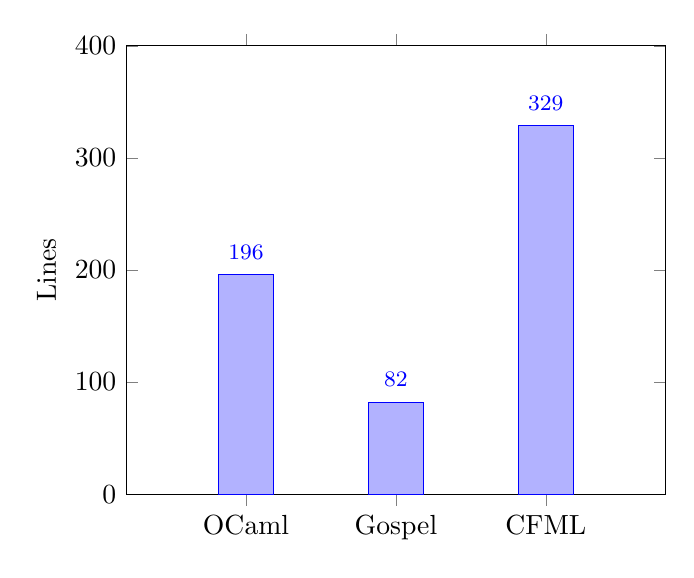
\begin{tikzpicture}
\begin{axis}[
    ybar,
    ymin=0,         % minimum value for y-axis
    ymax=400,       % maximum value for y-axis
    enlarge x limits=0.4,
    bar width=20pt,
    legend style={at={(0.5,-0.15)},
      anchor=north,legend columns=-1,},
    ylabel={Lines},
    symbolic x coords={OCaml, Gospel, CFML},
    xtick=data,
    x tick label style={ align=center},
    ]
    \addplot+[
    nodes near coords,
    every node near coord/.append style={font=\footnotesize, yshift=2pt}
] coordinates {
    (OCaml,196) (Gospel,82) (CFML,329)
};
\end{axis}
\end{tikzpicture}
\end{frame}


\section{Implementation}

\begin{frame}
  \vfill
  \centering
  {\Huge \textcolor{blue!70}{\textbf{Implementation}}}
  \vfill
\end{frame}

\section{Conclusion and Related Work}

\begin{frame}
  \vfill
  \centering
  {\Huge \textcolor{blue!70}{\textbf{Conclusion and Related Work}}}
  \vfill
\end{frame}

\begin{frame}{Conclusions}
  \begin{itemize}
    \item Designed and implemented a circular doubly linked list in OCaml.
    \item Verified key operations (such as \texttt{create},
      \texttt{clear}, \texttt{iter\_left}, \texttt{fold\_left}) using
      CFML.
    \item Demonstrated feasibility of verifying mutable data
      structures in a functional language.
    \item Identified limitations within the current toolchain.
  \end{itemize}
\end{frame}

\begin{frame}{Reflections \& Future Work}

  {\large \textbf{Reflections}}

  \begin{itemize}
      \item Formal verification remains time-intensive (some proofs may take months).
    \item Highlights both promise and current challenges in formally verifying real-world functional code.
    \end{itemize}

    \vspace{2em}

   {\large \textbf{Future Work}}
  \begin{itemize}
    \item Verify the remaining operations and auxiliary lemmas.
    \item Perform the refinement by comparing manual specs with
      Peter-generated ones.
      \end{itemize}
\end{frame}

\section{}

\begin{frame}[allowframebreaks, plain]{Bibliography}
  \nocite{*}
  \printbibliography[heading=none]
\end{frame}


\end{document}